\section {Problems and workaround}
Here we will talk about various problems we discovered during the soldering process, and how we found ways to workaround them.
We expect that there will be some things that may be possible to work around in code on the microcontroller, and other parts that require hardware fixes.
There might also be problems that cause parts of the board to not function.

\subsection{ Power connector footprint }

The footprint of the power connector had three pairs of holes instead of a milled groove.
This caused the connector to not fit in the footprint.
This was however solved by cutting away the parts of the connector that did not fit on the PCB using pliers.
The result worked fine, and it's hard to spot that the power connector is modified if you do not have a correctly mounted connector as a reference.

\subsection{ FPGA to SCU bus routing }

Because of an error made during the routing of the board, the header pin for FPGA\_ENABLE is not connected to any FPGA pins.
This error can be corrected by using one of our spare FPGA lines available on headers.
A wire was pulled from FPGA\_HEADER78 to the header from the SCU, and this header cable allowed us to run the rest of the bus as planed.

\subsection{ USB port }

\begin{figure}
\centering
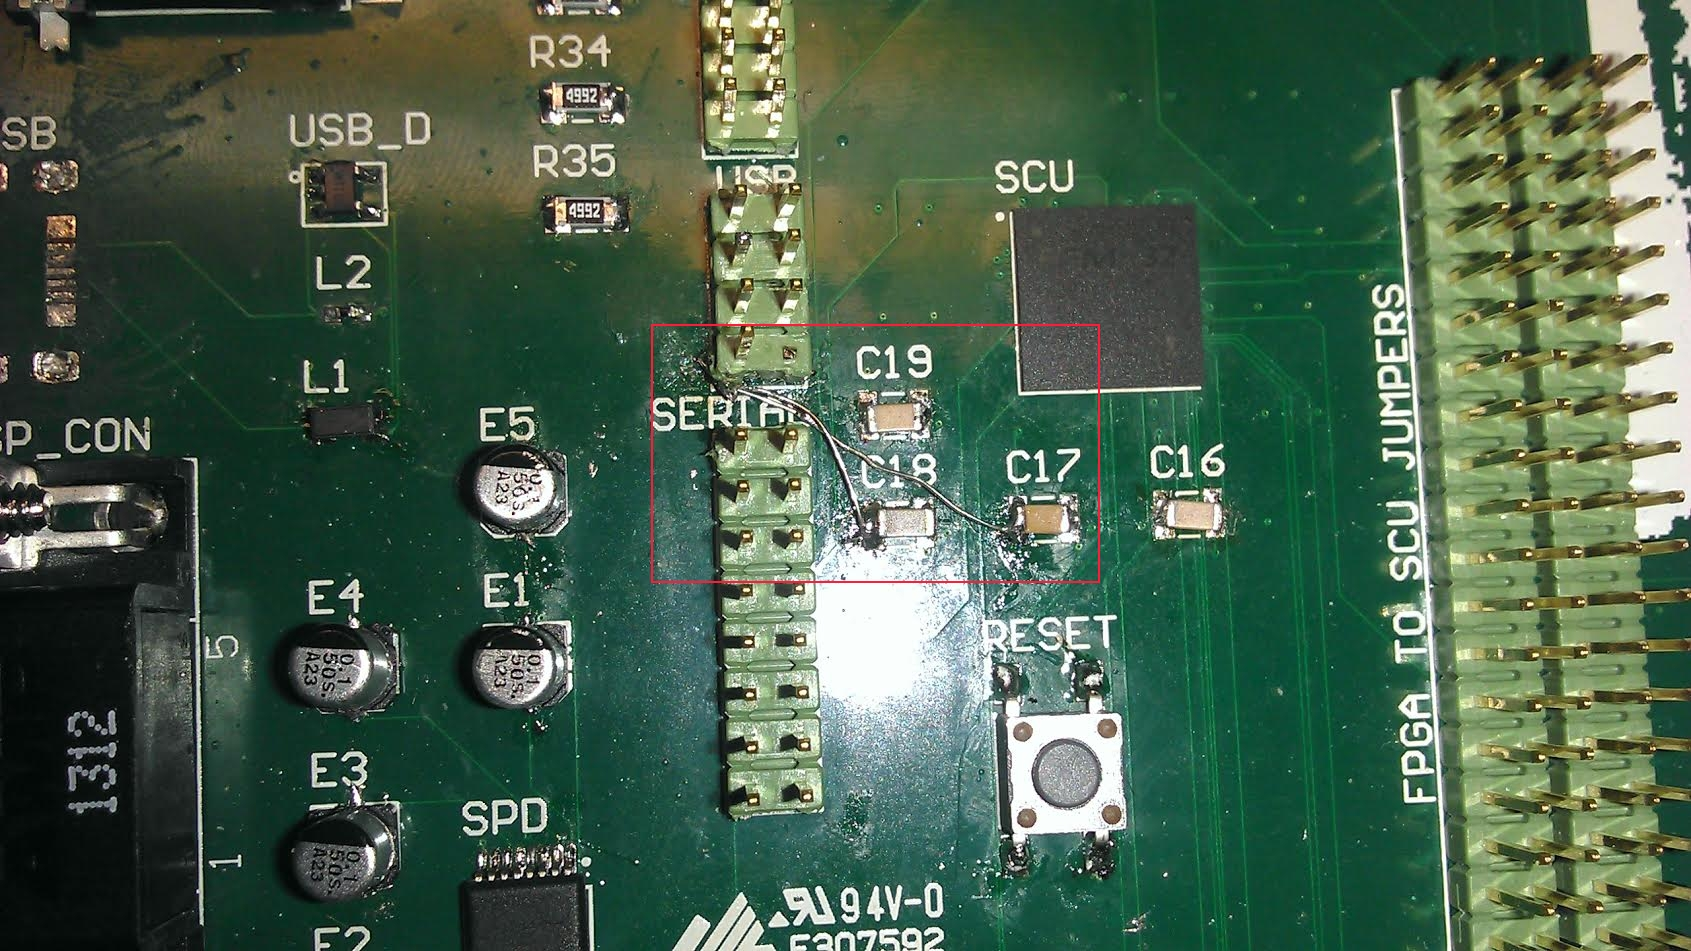
\includegraphics[width=5cm,keepaspectratio]{pcb/vreghack.jpeg}
\caption{The figure shows the "hack" that were made on the PCB in an attempt to fix the USB. Sadly the board were accidentally shortcircuted and died before this the hack could be fully verified to be working}
\label{figure:vreghack}
\end{figure}

When the PCB came back from production, it was discovered that the USB was not connected to the microcontroller
according to the recommended specifications from the manufacturer of the microcontroller. 
The problem was that the signals USB\_VBUS and USB\_VREGI were not connected to the VBUS-pin on the USB receptacle. This was fixed by soldering copper wires on the capacitators designated as C18 and C17 to USB-HEADER2 (called VBUS\_ENABLE in the schematics).
According to tests performed on the PCB before and after this work-around, the problem was fixed successfully.
